% ============================================================
% 第11章 三角形 — 人教版八年级上册
% 编译命令：xelatex -interaction=nonstopmode 第11章_三角形.tex
% ============================================================
\documentclass[12pt, a4paper]{ctexart}
\usepackage[margin=2.2cm]{geometry}
\usepackage{amsmath, amssymb}
\usepackage{enumitem}
\usepackage{tcolorbox}
\usepackage{booktabs}
\usepackage{array}
\usepackage{fancyhdr}
\usepackage{xcolor}
\usepackage{tikz}
\usepackage{hyperref}
\usepackage{graphicx}
\usepackage{multirow}
\usepackage{pgfplots}
\pgfplotsset{compat=1.18}

% 颜色定义
\definecolor{mainblue}{RGB}{41, 98, 168}
\definecolor{lightblue}{RGB}{230, 240, 255}
\definecolor{tipgreen}{RGB}{34, 139, 87}
\definecolor{lightgreen}{RGB}{235, 250, 240}
\definecolor{warnred}{RGB}{200, 50, 50}
\definecolor{lightred}{RGB}{255, 240, 240}
\definecolor{examorange}{RGB}{210, 120, 20}
\definecolor{lightorange}{RGB}{255, 248, 235}
\definecolor{apppurple}{RGB}{120, 60, 170}
\definecolor{lightpurple}{RGB}{245, 238, 255}

% 页眉页脚
\pagestyle{fancy}
\fancyhf{}
\fancyhead[L]{\small\textcolor{mainblue}{\textbf{人教版八年级上册 · 第11章 三角形}}}
\fancyhead[R]{\small\textcolor{mainblue}{三角形讲义}}
\fancyfoot[C]{\small —\ \thepage\ —}
\renewcommand{\headrulewidth}{0.6pt}
\renewcommand{\headrule}{\hbox to\headwidth{\color{mainblue}\leaders\hrule height \headrulewidth\hfill}}
\renewcommand{\footrulewidth}{0pt}

% tcolorbox 样式
\newtcolorbox{knowledgebox}[1][]{%
  colback=lightblue, colframe=mainblue,
  fonttitle=\bfseries\large, title=#1,
  arc=3mm, boxrule=0.8pt,
  left=8pt, right=8pt, top=6pt, bottom=6pt
}

\newtcolorbox{tipbox}[1][]{%
  colback=lightgreen, colframe=tipgreen,
  fonttitle=\bfseries, title=#1,
  arc=2mm, boxrule=0.6pt,
  left=6pt, right=6pt, top=4pt, bottom=4pt
}

\newtcolorbox{warnbox}[1][]{%
  colback=lightred, colframe=warnred,
  fonttitle=\bfseries, title=#1,
  arc=2mm, boxrule=0.6pt,
  left=6pt, right=6pt, top=4pt, bottom=4pt
}

\newtcolorbox{examplebox}[1][]{%
  colback=lightorange, colframe=examorange,
  fonttitle=\bfseries, title=#1,
  arc=3mm, boxrule=0.8pt,
  left=8pt, right=8pt, top=6pt, bottom=6pt
}

\newtcolorbox{appbox}[1][]{%
  colback=lightpurple, colframe=apppurple,
  fonttitle=\bfseries, title=#1,
  arc=3mm, boxrule=0.8pt,
  left=8pt, right=8pt, top=6pt, bottom=6pt
}

\setCJKmainfont{Hiragino Sans GB}
\setCJKsansfont{Heiti SC}

\begin{document}

% ============ 标题页 ============
\begin{center}
{\Huge\bfseries\textcolor{mainblue}{第11章\quad 三角形}}\\[12pt]
{\Large\textcolor{gray}{讲\quad 义}}\\[8pt]
\rule{0.6\textwidth}{1pt}\\[8pt]
{\normalsize 适用：人教版\quad 八年级上册\quad |\quad 课时：6课时}
\end{center}
\vspace{10pt}

% ============================================================
%  第一部分：知识点讲解
% ============================================================
\section*{\textcolor{mainblue}{一、知识点讲解}}

% ---- 11.1 三角形的边 ----
\subsection*{11.1\quad 三角形的边}

\begin{knowledgebox}[三角形的定义与基本要素]
\textbf{定义：}由不在同一直线上的三条线段首尾顺次相接所组成的图形叫做三角形。

基本要素：
\begin{itemize}[nosep]
  \item \textbf{顶点：}三角形有三个顶点，通常用大写字母 $A$、$B$、$C$ 表示，记作 $\triangle ABC$。
  \item \textbf{边：}三角形有三条边，分别是 $AB$、$BC$、$CA$（或 $a$、$b$、$c$）。
  \item \textbf{角：}三角形有三个内角，分别是 $\angle A$、$\angle B$、$\angle C$。
\end{itemize}
\end{knowledgebox}

\begin{knowledgebox}[三角形的三边关系]
\textbf{定理：}三角形两边之和大于第三边，两边之差小于第三边。

若三角形三边长分别为 $a$、$b$、$c$，则：
\[
a + b > c, \quad a + c > b, \quad b + c > a
\]
\[
|a - b| < c, \quad |a - c| < b, \quad |b - c| < a
\]
\end{knowledgebox}

\begin{warnbox}[易错提醒]
\textbf{判断三条线段能否构成三角形时，只需验证：}较短的两条边之和是否大于最长边。不必逐一验证三个不等式，只需抓住最长边这一关键即可。
\end{warnbox}

\begin{tipbox}[技巧]
已知三角形两边长为 $a$、$b$（设 $a \leqslant b$），则第三边 $c$ 的取值范围为：
\[
b - a < c < a + b
\]
\end{tipbox}

% ---- 11.2 三角形的角 ----
\subsection*{11.2\quad 三角形的角}

\begin{knowledgebox}[三角形内角和定理]
\textbf{定理：}三角形三个内角的和等于 $180°$。

即：$\angle A + \angle B + \angle C = 180°$。

\begin{center}
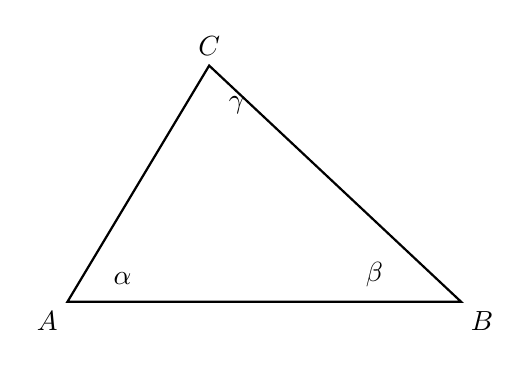
\begin{tikzpicture}[scale=1.0]
  \coordinate (A) at (0,0);
  \coordinate (B) at (5,0);
  \coordinate (C) at (1.8,3);
  \draw[thick] (A)--(B)--(C)--cycle;
  \node[below left] at (A) {$A$};
  \node[below right] at (B) {$B$};
  \node[above] at (C) {$C$};
  \node at (0.7,0.3) {$\alpha$};
  \node at (3.9,0.35) {$\beta$};
  \node at (2.15,2.5) {$\gamma$};
\end{tikzpicture}
\end{center}

证明思路：过顶点 $A$ 作 $BC$ 的平行线，利用平行线的性质（内错角相等）和邻补角关系，可得三角和为平角 $180°$。
\end{knowledgebox}

\begin{knowledgebox}[三角形外角定理]
\textbf{定义：}三角形的一边与另一边的延长线组成的角，叫做三角形的外角。

\textbf{定理：}
\begin{enumerate}[nosep]
  \item 三角形的一个外角等于与它不相邻的两个内角之和。
  \item 三角形的一个外角大于任何一个与它不相邻的内角。
\end{enumerate}

\begin{center}
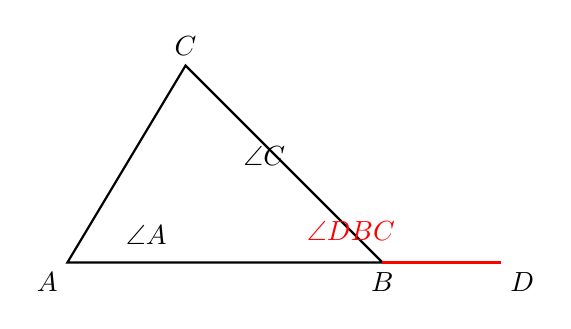
\begin{tikzpicture}[scale=1.0]
  \coordinate (A) at (0,0);
  \coordinate (B) at (4,0);
  \coordinate (C) at (1.5,2.5);
  \coordinate (D) at (5.5,0);
  \draw[thick] (A)--(B)--(C)--cycle;
  \draw[thick, red] (B)--(D);
  \node[below left] at (A) {$A$};
  \node[below] at (B) {$B$};
  \node[above] at (C) {$C$};
  \node[below right] at (D) {$D$};
  \node at (1.0,0.35) {$\angle A$};
  \node at (2.5,1.35) {$\angle C$};
  \node at (3.6,0.4) {$\color{red}\angle DBC$};
\end{tikzpicture}
\end{center}

如上图，$\angle DBC = \angle A + \angle C$（外角等于不相邻两内角之和）。
\end{knowledgebox}

\begin{warnbox}[易错提醒]
\textbf{外角和是每一个顶点处只取一个外角！}三角形有六个外角（每个顶点两个），但外角和是指每个顶点取一个，共三个外角之和为 $360°$。切勿将六个外角相加。
\end{warnbox}

% ---- 11.3 三角形的分类 ----
\subsection*{11.3\quad 三角形的分类}

\begin{knowledgebox}[按角分类]
\begin{itemize}[nosep]
  \item \textbf{锐角三角形：}三个内角都是锐角（均小于 $90°$）。
  \item \textbf{直角三角形：}有一个内角是直角（等于 $90°$）。直角所对的边叫做斜边。
  \item \textbf{钝角三角形：}有一个内角是钝角（大于 $90°$ 小于 $180°$）。
\end{itemize}
\begin{center}
\begin{tikzpicture}[scale=0.8]
  % 锐角三角形
  \draw[thick] (0,0)--(2,0)--(0.8,1.5)--cycle;
  \node[below] at (1,0) {\small 锐角三角形};
  % 直角三角形
  \draw[thick] (3.5,0)--(5.5,0)--(3.5,2)--cycle;
  \draw (3.5,0.3)--(3.8,0.3)--(3.8,0);
  \node[below] at (4.5,0) {\small 直角三角形};
  % 钝角三角形
  \draw[thick] (7,0)--(9.5,0)--(6.5,1.2)--cycle;
  \node[below] at (8,0) {\small 钝角三角形};
\end{tikzpicture}
\end{center}
\end{knowledgebox}

\begin{knowledgebox}[按边分类]
\begin{itemize}[nosep]
  \item \textbf{不等边三角形：}三条边互不相等。
  \item \textbf{等腰三角形：}有两条边相等。相等的两边叫做腰，第三边叫做底边。
  \item \textbf{等边三角形（正三角形）：}三条边都相等。等边三角形是特殊的等腰三角形。
\end{itemize}
\end{knowledgebox}

% ---- 11.4 三角形的高、中线、角平分线 ----
\subsection*{11.4\quad 三角形的高、中线与角平分线}

\begin{knowledgebox}[三角形的高]
\textbf{定义：}从三角形的一个顶点向它的对边所在直线作垂线，顶点和垂足之间的线段叫做三角形的高。

\begin{itemize}[nosep]
  \item 三角形有三条高。
  \item 锐角三角形的三条高都在三角形内部。
  \item 直角三角形有两条高恰好是两条直角边。
  \item 钝角三角形有两条高在三角形外部。
\end{itemize}

\begin{center}
\begin{tikzpicture}[scale=0.75]
  % 锐角三角形的高
  \coordinate (A1) at (0,0);
  \coordinate (B1) at (3.5,0);
  \coordinate (C1) at (1.2,2.5);
  \coordinate (H1) at (1.2,0);
  \draw[thick] (A1)--(B1)--(C1)--cycle;
  \draw[blue, dashed] (C1)--(H1);
  \draw (1.2,0.25)--(1.45,0.25)--(1.45,0);
  \node[below] at (1.75,-0.5) {\small 锐角三角形};

  % 直角三角形的高
  \coordinate (A2) at (5.5,0);
  \coordinate (B2) at (8.5,0);
  \coordinate (C2) at (5.5,2.2);
  \draw[thick] (A2)--(B2)--(C2)--cycle;
  \draw (5.5,0.25)--(5.75,0.25)--(5.75,0);
  \node[below] at (7,-0.5) {\small 直角三角形};
\end{tikzpicture}
\end{center}
\end{knowledgebox}

\begin{knowledgebox}[三角形的中线]
\textbf{定义：}连接三角形一个顶点和它对边中点的线段叫做三角形的中线。

\begin{itemize}[nosep]
  \item 三角形有三条中线，它们都在三角形内部。
  \item 三条中线交于一点，叫做\textbf{重心}。
  \item 重心到顶点的距离等于它到对边中点距离的2倍。
\end{itemize}
\end{knowledgebox}

\begin{knowledgebox}[三角形的角平分线]
\textbf{定义：}三角形一个角的平分线与这个角的对边相交，顶点和交点之间的线段叫做三角形的角平分线。

\begin{itemize}[nosep]
  \item 三角形有三条角平分线，它们都在三角形内部。
  \item 三条角平分线交于一点，叫做\textbf{内心}，是三角形内切圆的圆心。
\end{itemize}
\end{knowledgebox}

% ---- 11.5 三角形的稳定性 ----
\subsection*{11.5\quad 三角形的稳定性}

\begin{knowledgebox}[三角形的稳定性]
三角形的三边长度确定后，三角形的形状和大小就唯一确定了。这种性质叫做\textbf{三角形的稳定性}。

\textbf{应用举例：}
\begin{itemize}[nosep]
  \item 三角形支架（如桥梁、屋顶桁架）
  \item 自行车车架
  \item 照相机三脚架
\end{itemize}

\textbf{对比：}四边形不具有稳定性，容易变形。但可以通过添加对角线（构成三角形）来增强稳定性。
\end{knowledgebox}

% ---- 11.6 多边形 ----
\subsection*{11.6\quad 多边形的内角和与外角和}

\begin{knowledgebox}[多边形的内角和]
$n$ 边形（$n \geqslant 3$）的内角和公式：
\[
\boxed{S = (n - 2) \times 180°}
\]

\textbf{推导方法：}从 $n$ 边形的一个顶点出发，可以引 $(n-3)$ 条对角线，将 $n$ 边形分成 $(n-2)$ 个三角形。每个三角形内角和为 $180°$，所以 $n$ 边形内角和为 $(n-2) \times 180°$。

\begin{center}
\begin{tikzpicture}[scale=0.9]
  % 五边形
  \foreach \i in {1,...,5}{
    \coordinate (P\i) at ({90+(\i-1)*72}:1.5);
  }
  \draw[thick] (P1)--(P2)--(P3)--(P4)--(P5)--cycle;
  \draw[dashed, blue] (P1)--(P3);
  \draw[dashed, blue] (P1)--(P4);
  \node[above] at (P1) {$A_1$};
  \node[right] at (P2) {$A_2$};
  \node[below right] at (P3) {$A_3$};
  \node[below left] at (P4) {$A_4$};
  \node[left] at (P5) {$A_5$};
  \node at (0,-2.3) {\small 五边形内角和 $= 3 \times 180° = 540°$};
\end{tikzpicture}
\end{center}
\end{knowledgebox}

\begin{knowledgebox}[多边形的外角和]
任意多边形的外角和等于 $360°$：
\[
\boxed{\text{外角和} = 360°}
\]

不论边数 $n$ 是多少，外角和恒为 $360°$。
\end{knowledgebox}

\begin{warnbox}[易错提醒]
\textbf{正多边形每个内角}的度数为 $\dfrac{(n-2) \times 180°}{n}$，每个外角的度数为 $\dfrac{360°}{n}$。不要把"内角和"与"每个内角"混淆！
\end{warnbox}

\begin{tipbox}[规律]
\begin{itemize}[nosep]
  \item 正三角形每个内角 $60°$；正方形每个内角 $90°$；正六边形每个内角 $120°$。
  \item 若一个多边形的每个外角都是 $40°$，则边数 $n = 360° \div 40° = 9$。
\end{itemize}
\end{tipbox}

% ============================================================
%  第二部分：例题精讲
% ============================================================
\section*{\textcolor{examorange}{二、例题精讲}}

\begin{examplebox}[【例题1】基础计算——求三角形第三边的取值范围]
已知三角形的两边长分别为 $3$ 和 $7$，求第三边 $x$ 的取值范围。
\end{examplebox}

\textbf{解：}

由三角形三边关系，第三边 $x$ 满足：
\[
7 - 3 < x < 7 + 3
\]
\[
4 < x < 10
\]

所以第三边的取值范围为 $4 < x < 10$。

\begin{tipbox}[方法总结]
已知两边求第三边的范围：设已知两边 $a \leqslant b$，则第三边 $c$ 满足 $b - a < c < a + b$。记住口诀："两边之差小于第三边，两边之和大于第三边"。
\end{tipbox}

\begin{examplebox}[【例题2】基础计算——利用内角和求角]
在 $\triangle ABC$ 中，$\angle A = 50°$，$\angle B = 2\angle C$，求 $\angle B$ 和 $\angle C$ 的度数。
\end{examplebox}

\textbf{解：}

设 $\angle C = x$，则 $\angle B = 2x$。

由三角形内角和定理：
\[
\angle A + \angle B + \angle C = 180°
\]
\[
50° + 2x + x = 180°
\]
\[
3x = 130°
\]
\[
x = \frac{130°}{3} = 43\frac{1}{3}°
\]

所以 $\angle C = 43\dfrac{1}{3}°$，$\angle B = 86\dfrac{2}{3}°$。

\begin{tipbox}[方法总结]
遇到"内角和"问题，核心方程就是 $\angle A + \angle B + \angle C = 180°$。如果角之间有倍数关系，设未知数列方程求解。
\end{tipbox}

\begin{examplebox}[【例题3】几何证明——外角定理的应用]
如图，已知 $D$ 是 $\triangle ABC$ 的边 $BC$ 延长线上一点，$\angle A = 55°$，$\angle B = 40°$。求 $\angle ACD$ 的度数，并说明理由。

\begin{center}
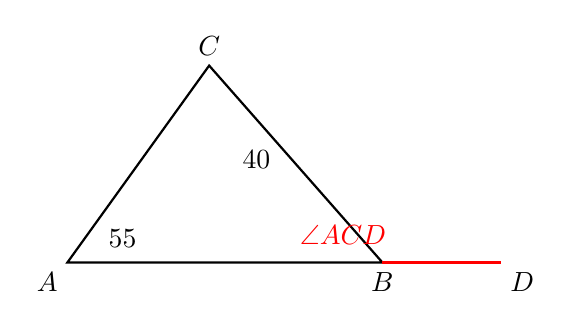
\begin{tikzpicture}[scale=1.0]
  \coordinate (A) at (0,0);
  \coordinate (B) at (4,0);
  \coordinate (C) at (1.8,2.5);
  \coordinate (D) at (5.5,0);
  \draw[thick] (A)--(B)--(C)--cycle;
  \draw[thick, red] (B)--(D);
  \node[below left] at (A) {$A$};
  \node[below] at (B) {$B$};
  \node[above] at (C) {$C$};
  \node[below right] at (D) {$D$};
  \node at (0.7,0.3) {$55°$};
  \node at (3.5,0.35) {$\color{red}\angle ACD$};
  \node at (2.4,1.3) {$40°$};
\end{tikzpicture}
\end{center}
\end{examplebox}

\textbf{解：}

\textbf{已知：}$D$ 在 $BC$ 的延长线上，$\angle A = 55°$，$\angle B = 40°$。

\textbf{求：}$\angle ACD$ 的度数。

\textbf{解法一（利用外角定理）：}

$\angle ACD$ 是 $\triangle ABC$ 的一个外角，它等于与它不相邻的两个内角之和：
\[
\angle ACD = \angle A + \angle B = 55° + 40° = 95°
\]

\textbf{解法二（利用内角和）：}

先求 $\angle C$：
\[
\angle C = 180° - \angle A - \angle B = 180° - 55° - 40° = 85°
\]
再由邻补角关系：
\[
\angle ACD = 180° - \angle C = 180° - 85° = 95°
\]

\begin{tipbox}[方法总结]
求三角形外角有两种方法：(1) 直接用外角定理（外角 $=$ 不相邻两内角之和），更快；(2) 先求内角再用补角关系。推荐方法一。
\end{tipbox}

\begin{examplebox}[【例题4】易错辨析——判断三边能否构成三角形]
以下各组线段中，能构成三角形的是（\quad）

A.\ $1, 2, 3$ \quad B.\ $2, 3, 6$ \quad C.\ $3, 4, 5$ \quad D.\ $2, 2, 5$
\end{examplebox}

\textbf{解：}

逐项验证"较短两边之和是否大于最长边"：

\begin{itemize}[nosep]
  \item A：$1 + 2 = 3$，不大于 $3$，\textbf{不能}构成三角形。
  \item B：$2 + 3 = 5 < 6$，\textbf{不能}构成三角形。
  \item C：$3 + 4 = 7 > 5$，\textbf{能}构成三角形。
  \item D：$2 + 2 = 4 < 5$，\textbf{不能}构成三角形。
\end{itemize}

答案选 \textbf{C}。

\begin{warnbox}[易错提醒]
注意 A 选项：$1 + 2 = 3$ 恰好等于第三边，这种情况三点共线，\textbf{不能}构成三角形！必须严格"大于"，不能"大于等于"。
\end{warnbox}

\begin{examplebox}[【例题5】综合提高——等腰三角形的周长问题]
已知等腰三角形的两边长分别为 $4$ 和 $9$，求该三角形的周长。
\end{examplebox}

\textbf{解：}

需要分两种情况讨论：

\textbf{情况一：腰长为 $4$，底边为 $9$。}

此时三边为 $4, 4, 9$。

验证：$4 + 4 = 8 < 9$，不满足"两边之和大于第三边"，\textbf{不能}构成三角形。

\textbf{情况二：腰长为 $9$，底边为 $4$。}

此时三边为 $9, 9, 4$。

验证：$9 + 4 = 13 > 9$，满足三边关系，\textbf{能}构成三角形。

所以周长为 $9 + 9 + 4 = 22$。

\begin{tipbox}[方法总结]
等腰三角形分类讨论时，求出两种情况后\textbf{必须逐一验证}是否满足三边关系！很多同学忘记了验证，导致多解。
\end{tipbox}

\begin{examplebox}[【例题6】综合提高——多边形内角和与外角和]
一个正多边形的每个内角都等于 $135°$，求这个正多边形的边数。
\end{examplebox}

\textbf{解：}

\textbf{方法一（用内角和公式）：}

设边数为 $n$，正多边形每个内角为 $\dfrac{(n-2) \times 180°}{n}$。

\[
\frac{(n-2) \times 180°}{n} = 135°
\]
\[
(n-2) \times 180 = 135n
\]
\[
180n - 360 = 135n
\]
\[
45n = 360
\]
\[
n = 8
\]

\textbf{方法二（用外角和）：}

每个外角 $= 180° - 135° = 45°$。

\[
n = \frac{360°}{45°} = 8
\]

所以这个正多边形是正八边形。

\begin{tipbox}[方法总结]
涉及正多边形每个内角/外角的问题，用外角和公式 $n = 360° \div \text{每个外角}$ 往往更简洁，避免解方程。
\end{tipbox}

\begin{examplebox}[【例题7】与代数交叉的综合题]
已知三角形三边长分别为 $a$、$b$、$c$，且满足 $|a - 3| + (b - 4)^2 + \sqrt{c - 5} = 0$。判断 $\triangle ABC$ 的形状。
\end{examplebox}

\textbf{解：}

因为 $|a - 3| \geqslant 0$，$(b - 4)^2 \geqslant 0$，$\sqrt{c - 5} \geqslant 0$，且三者之和为 $0$，所以：
\[
|a - 3| = 0, \quad (b - 4)^2 = 0, \quad \sqrt{c - 5} = 0
\]
\[
a = 3, \quad b = 4, \quad c = 5
\]

验证三边关系：$3 + 4 = 7 > 5$，能构成三角形。

又因为 $3^2 + 4^2 = 9 + 16 = 25 = 5^2$，即 $a^2 + b^2 = c^2$，

所以 $\triangle ABC$ 是直角三角形（勾股定理的逆定理）。

\begin{tipbox}[方法总结]
绝对值、完全平方、算术平方根三者非负性结合为零，是代数中的经典题型。求出三边后，再用几何知识判断形状。
\end{tipbox}

% ============================================================
%  第三部分：应用题
% ============================================================
\section*{\textcolor{apppurple}{三、应用题}}

\begin{appbox}[【应用1】建筑中的三角形稳定性]
小明家要装修房子，工人师傅在墙上安装一个三角形支架来固定搁板。已知墙面和搁板互相垂直，支架的两条边分别长 $30\text{ cm}$ 和 $40\text{ cm}$，且紧贴墙面和搁板。请问第三条边（斜撑）的长度是多少厘米？如果搁板上放了重物后，斜撑受力，这个三角形为什么不容易变形？
\end{appbox}

\textbf{解：}

墙面与搁板垂直，所以支架构成一个直角三角形，两条直角边分别为 $30\text{ cm}$ 和 $40\text{ cm}$。

由勾股定理（后续章节详细学习），斜边为：
\[
c = \sqrt{30^2 + 40^2} = \sqrt{900 + 1600} = \sqrt{2500} = 50 \text{ cm}
\]

斜撑长 $50\text{ cm}$。

三角形具有\textbf{稳定性}——当三条边的长度确定后，三角形的形状就完全确定，不会发生变形。这就是为什么建筑、桥梁等结构中广泛使用三角形支架的原因。

\begin{appbox}[【应用2】测量中的三角形内角和]
如图，小华站在点 $A$ 处观测远处的山顶 $C$ 和山脚 $B$。已知 $\angle CAB = 35°$，小华沿着水平方向走到点 $B$（山脚），再测得 $\angle ABC = 100°$。请问山顶处的视角 $\angle ACB$ 是多少度？

\begin{center}
\begin{tikzpicture}[scale=0.9]
  \coordinate (A) at (0,0);
  \coordinate (B) at (5,0);
  \coordinate (C) at (2.3,3);
  \draw[thick] (A)--(B)--(C)--cycle;
  \node[below left] at (A) {$A$（观测点）};
  \node[below right] at (B) {$B$（山脚）};
  \node[above] at (C) {$C$（山顶）};
  \node at (1.0,0.3) {$35°$};
  \node at (4.1,0.45) {$100°$};
  \node at (2.6,2.4) {$?$};
\end{tikzpicture}
\end{center}
\end{appbox}

\textbf{解：}

在 $\triangle ABC$ 中，由三角形内角和定理：
\[
\angle ACB = 180° - \angle CAB - \angle ABC = 180° - 35° - 100° = 45°
\]

所以山顶处的视角 $\angle ACB = 45°$。

\begin{appbox}[【应用3】正多边形铺地砖]
小红家要装修客厅地面，她想用正多边形的地砖进行无缝铺贴（不留缝隙、不重叠）。请问她可以选择哪些正多边形的地砖？请说明理由。
\end{appbox}

\textbf{解：}

无缝铺贴要求在每一个拼接点处，若干块地砖的内角之和恰好为 $360°$。

设正 $n$ 边形的每个内角为 $\alpha$，则：
\[
\alpha = \frac{(n-2) \times 180°}{n}
\]

要使 $k$ 块相同的正 $n$ 边形地砖拼在一个点处不留缝隙，需要 $k \cdot \alpha = 360°$，即 $k = \dfrac{360°}{\alpha}$ 必须是正整数。

\begin{itemize}[nosep]
  \item 正三角形：$\alpha = 60°$，$k = 360° / 60° = 6$（整数，可行）
  \item 正方形：$\alpha = 90°$，$k = 360° / 90° = 4$（整数，可行）
  \item 正五边形：$\alpha = 108°$，$k = 360° / 108° = 3.33\ldots$（不是整数，不可行）
  \item 正六边形：$\alpha = 120°$，$k = 360° / 120° = 3$（整数，可行）
  \item 正七边形及以上：$\alpha > 120°$，$k < 3$，且 $360° / \alpha$ 不是整数，不可行。
\end{itemize}

所以小红可以选择正三角形、正方形或正六边形的地砖。

% ============================================================
%  第四部分：课堂练习
% ============================================================
\section*{\textcolor{tipgreen}{四、课堂练习}}

\begin{enumerate}
  \item 已知三角形的两边长分别为 $5$ 和 $8$，若第三边为偶数，求第三边的所有可能值。

  \item 在 $\triangle ABC$ 中，$\angle A : \angle B : \angle C = 2 : 3 : 5$，求三个内角的度数。

  \item 一个多边形的内角和为 $1260°$，求它的边数。

  \item 已知等腰三角形的一边长为 $6$，另一边长为 $13$，求它的周长。

  \item 如图，$D$ 是 $\triangle ABC$ 边 $BC$ 上一点，$\angle ADC = 80°$，$\angle B = 45°$，$\angle BAD = \angle DAC$，求 $\angle C$ 的度数。

\begin{center}
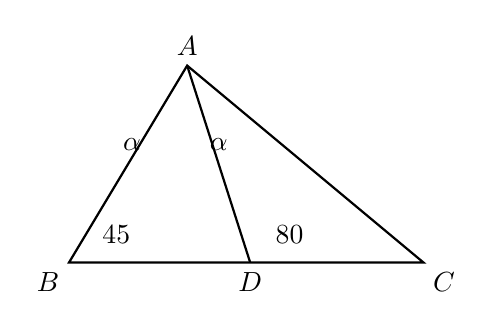
\begin{tikzpicture}[scale=1.0]
  \coordinate (A) at (0,2.5);
  \coordinate (B) at (-1.5,0);
  \coordinate (C) at (3,0);
  \coordinate (D) at (0.8,0);
  \draw[thick] (A)--(B)--(C)--cycle;
  \draw[thick] (A)--(D);
  \node[above] at (A) {$A$};
  \node[below left] at (B) {$B$};
  \node[below right] at (C) {$C$};
  \node[below] at (D) {$D$};
  \node at (-0.7,1.5) {$\alpha$};
  \node at (0.4,1.5) {$\alpha$};
  \node at (-0.9,0.35) {$45°$};
  \node at (1.3,0.35) {$80°$};
\end{tikzpicture}
\end{center}
\end{enumerate}

% ---- 参考答案 ----
\begin{knowledgebox}[参考答案]
\textbf{1.} 设第三边为 $c$，则 $8 - 5 < c < 8 + 5$，即 $3 < c < 13$。
又 $c$ 为偶数，所以 $c$ 的可能值为 $4, 6, 8, 10, 12$。

\medskip

\textbf{2.} 设 $\angle A = 2k$，$\angle B = 3k$，$\angle C = 5k$。
\[
2k + 3k + 5k = 180° \implies 10k = 180° \implies k = 18°
\]
所以 $\angle A = 36°$，$\angle B = 54°$，$\angle C = 90°$。

\medskip

\textbf{3.} 由 $(n - 2) \times 180° = 1260°$，得 $n - 2 = 7$，所以 $n = 9$，即九边形。

\medskip

\textbf{4.} 分两种情况：
\begin{itemize}[nosep]
  \item 若腰为 $6$，底为 $13$：$6 + 6 = 12 < 13$，不满足三边关系，舍去。
  \item 若腰为 $13$，底为 $6$：$13 + 6 = 19 > 13$，满足。周长 $= 13 + 13 + 6 = 32$。
\end{itemize}
所以等腰三角形的周长为 $32$。

\medskip

\textbf{5.} 在 $\triangle ABD$ 中，$\angle ADB = 180° - \angle ADC = 180° - 80° = 100°$。

由内角和：$\angle BAD = 180° - \angle B - \angle ADB = 180° - 45° - 100° = 35°$。

因为 $\angle BAD = \angle DAC = 35°$，所以 $\angle BAC = 70°$。

在 $\triangle ABC$ 中：$\angle C = 180° - \angle B - \angle BAC = 180° - 45° - 70° = 65°$。
\end{knowledgebox}

\vfill
\begin{center}
\small\textcolor{gray}{本讲义仅供教学参考，例题可根据学生水平调整难度。}
\end{center}

\end{document}
